%%%%%%%%%%%%%%%%%%%%%%%%%%%%%%%%%%%%%%%%%%%%%%%%%%%%%%%%%%%%%%%%%%%%%%
% LaTeX Example: Project Report
%
% Source: http://www.howtotex.com
%
%%%%%%%%%%%%%%%%%%%%%%%%%%%%%%%%%%%%%%%%%%%%%%%%%%%%%%%%%%%%%%%%%%%%%%


%%% Preamble
\documentclass[paper=a4, fontsize=11pt]{scrartcl}
\usepackage[T1]{fontenc}
\usepackage{fourier}

\usepackage[utf8]{inputenc}
\usepackage{polski}
\usepackage[protrusion=true,expansion=true]{microtype}	
\usepackage{amsmath,amsfonts,amsthm} % Math packages
\usepackage[pdftex]{graphicx}	
\usepackage{float}
\usepackage{url}
\usepackage[margin=2.5cm]{geometry}

%%% Custom sectioning
\usepackage{sectsty}
\allsectionsfont{\normalfont\scshape}


%%% Custom headers/footers (fancyhdr package)
\usepackage{fancyhdr}
\pagestyle{fancyplain}
\fancyhead{}											% No page header
\fancyfoot[L]{}											% Empty 
\fancyfoot[C]{}											% Empty
\fancyfoot[R]{\thepage}									% Pagenumbering
\renewcommand{\headrulewidth}{0pt}			% Remove header underlines
\renewcommand{\footrulewidth}{0pt}				% Remove footer underlines
\setlength{\headheight}{13.6pt}


%%% Equation and float numbering
\numberwithin{equation}{section}		% Equationnumbering: section.eq#
\numberwithin{figure}{section}			% Figurenumbering: section.fig#
\numberwithin{table}{section}				% Tablenumbering: section.tab#


%%% Maketitle metadata
\newcommand{\horrule}[1]{\rule{\linewidth}{#1}} 	% Horizontal rule

\title{
		%\vspace{-1in} 	
		\usefont{OT1}{bch}{b}{n}
		\normalfont \normalsize \textsc{Akademia Górniczo Hutnicza} \\ [25pt]
		Wydział Informatyki, Elektroniki i Telekomunikacji
		\horrule{0.5pt} \\[1cm]
		
\includegraphics[width=.35\textwidth]{img/agh_znk_wbr_cmyk.eps} \\[1.5cm]
		\huge System usprawniający deklarację i zbiórkę odpadów
		\horrule{0.5pt} \\[0cm]
}
\author{
		\normalfont \normalsize
        Mateusz Kwiecień\\[-3pt]	\normalsize
        Beata Obrok\\[-3pt]			\normalsize
        Arkadiusz Socha\\[-3pt]		\normalsize
        Dawid Suder\\[-3pt]			\normalsize
}
\date{}


%%% Begin document
\begin{document}
\maketitle
\tableofcontents

\section{Sformułowanie zadania projektowego}

	\subsection{Obszar i przedmiot modelowania}

		\subsubsection{Dziedzina problemu}
			
% Firma, cel, dziedzina, schemat struktury organizacyjnej, słownik pojęć biznesowych (lub odsyłacz do załącznika)
% Ogólne omówienie zakresu i charakteru działalności jednostki dla której przeznaczony jest produkt tj. realizowany [projektowany] system).
% Dołączyć i opisać schemat struktury organizacyjnej jednostki. 



	\subsection{Obszar modelowania}

		\subsubsection{Opis struktury organizacyjnej}
			
% Opisowy model stanu istniejącego
% Opis wszystkich składników organizacyjnych
% Związek struktury z dziedziną obszaru modelowania, wyznaczenie zakresu odpowiedzialności systemu 	

\textbf{Grupa Kapitałowa Biosystem} składa się z trzech podmiotów gospodarczych (\textbf{BIOSYSTEM S.A.}, \textbf{BIOSYSTEM ElektrorecyklingOrganizacja Odzysku Sprzętu Elektrycznego i Elektronicznego S.A.}, \textbf{Zakład Gospodarki Komunalnej Organizacja Odzysku BIOSYSTEM S.A.}. Firma \textbf{BIOSYSTEM S.A.} stanowi spółkę nadrzędną.

\begin{figure}[H]
	\centering
	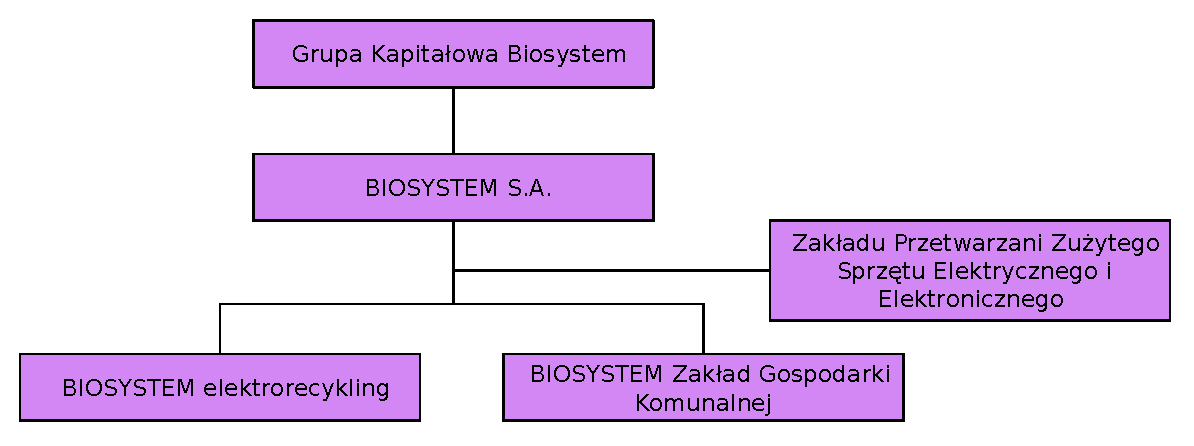
\includegraphics[width=\textwidth]{img/group_chart.eps}
	\caption{Struktura grupy kapitałowej}
\end{figure}


\begin{figure}[H]
    \centering
    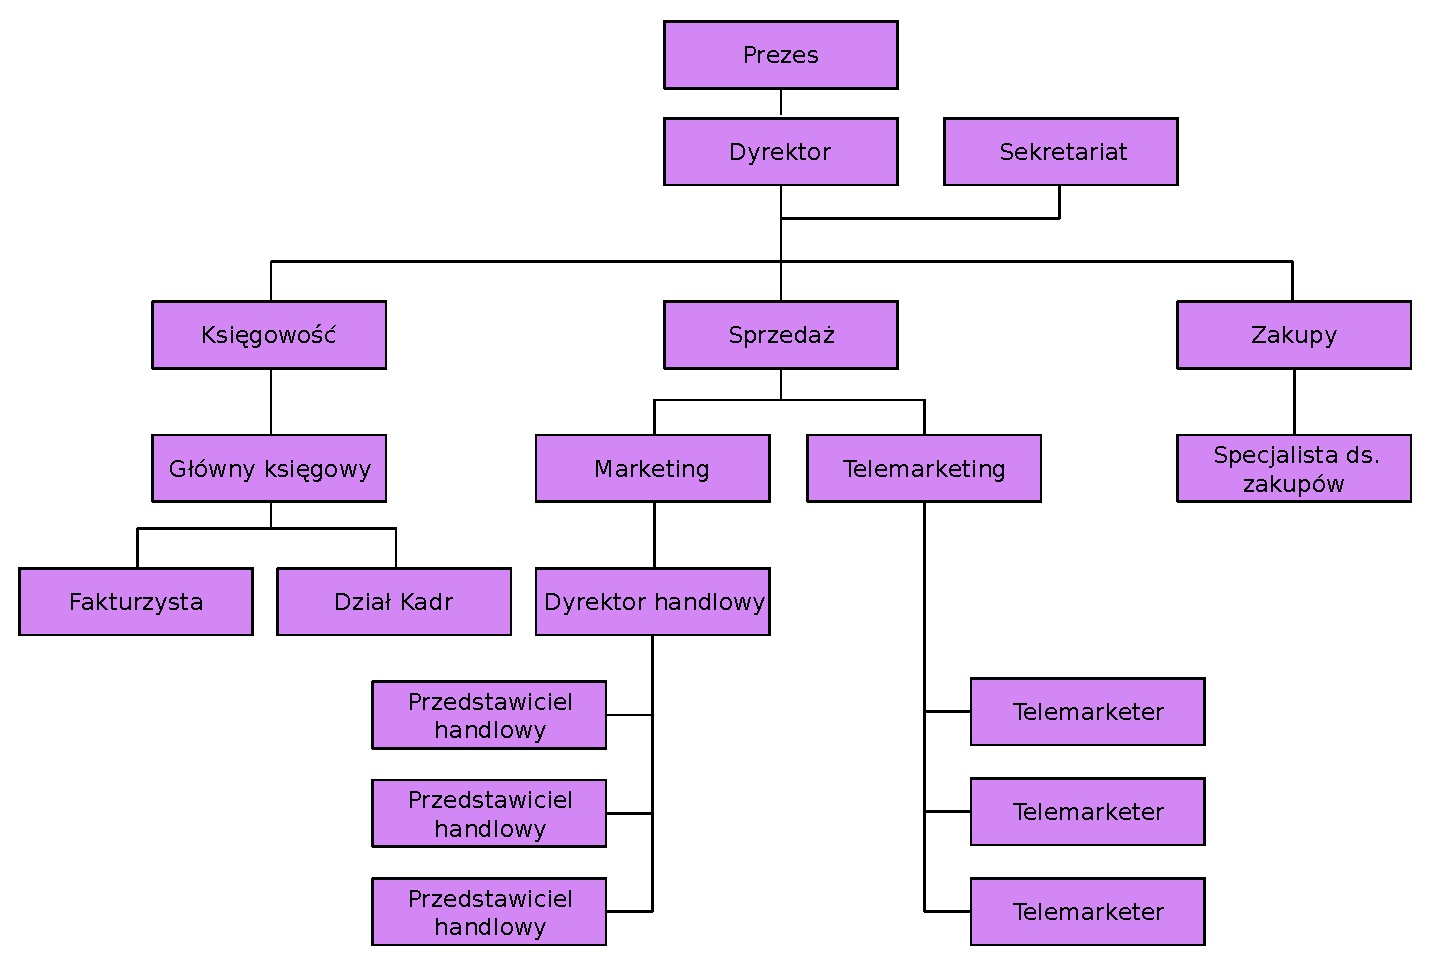
\includegraphics[width=1\textwidth]{img/organization_chart.eps}
    \caption{Struktura organizacyjna spółki}
\end{figure}

		\subsubsection{Obszary aktywności}
			
% Wyznaczenie obszarów aktywności, które będą omówione szczegółowo w kolejnym podrozdziale

\begin{figure}[H]
	\centering
	\caption{Obszary aktywności}
\end{figure}

\paragraph{Obszary aktywności} \ \\
\begin{itemize}
	\item Obsługa sprzedającego \\
	\paragraph 	Sprzedający może powiadomić firmę o posiadanych surowcach wtrórnych osobiście, telefonicznie, a także za pomocą strony internetowej. W zależności od ilości odpadów, a także od lokalizacji klienta, firma może wysłać kierowcę po ich odbiór, lub sprzedający może przywieźć je osobiście. Pieniądze są wpłacane na konto klienta do dwóch tygodni od odbioru towarów wtórnych.
	\item Obsługa kupującego \\
	\paragraph 	Kupujący składa zamówienie osobiście, telefonicznie, a także za pomocą strony internetwowej. Firma wysyła kierowcę z zamówieniem, a klient odpbiera je płacąc, za dowieziony towar, chyba, że wcześniej zapłacił za niego przelewem.
	\item Wspomaganie pracy kierowców \\
	\paragraph 	Kierowcy odbierają odpady od klientów z terenów Małopolski. Zabierają ze sobą potwierdzenie odbioru, którą wręczają sprzedającemu. Następnie przewożą odpady do:
		\begin{itemize}
			\item zewnętrznej firmy recyklingowej(opakowania z papieru, tworzyw sztucznych, szkła, blachy i aluminum),
			\item własnego zakładu przetwarzania sprzętu elektrycznego i elektronicznego.
		\end{itemize}
	Kierowcy zajmują sie także dostarczeniem zamówienia do kupującego. Zabierają ze sobą fakturę, którą wręczają kupującemu.
	\item Wspomaganie pracy magazynierów \\
	\paragraph Pracownicy magazynu grupują produkty otrzymane po recyklingu. Zajmują się także przygotowaniem 
	\item Wspomaganie pracy pracownika działu sprzedaży \\ 
	\paragraph 	Dział sprzedaży zajmuje się pozyskiwaniem klientów, którzy kupią odpady poddane już recyklingowi
\end{itemize}

	\subsection{Opis obszarów aktywności}

		\subsubsection{Opis stanowisk pracy}
			
\begin{enumerate}
	\item Właściciel \\ 
	Właściciel firmy odpowiada za jej funkcjonowanie, podlegają mu pracownicy. Do jego głównych zadań należą:
	\begin{itemize}
		\item organizacja pracy podwładnych i ustalanie wynagrodzenia
		\item nadzór nad spółkami zależnymi
	\end{itemize}
	\item Pracownik działu skupu \\
	Głównym jego zadaniem jest odebranie deklaracji o ilości odpoadów od sprzedającego, przygotowanie potwierdzenia odbioru, oraz przekazanie go kierowcy.
	\item Pracownicy działu sprzedaży
	\begin{itemize}
	\item Przedstawiciel handlowy \\
	Zajmuje się pozyskiwaniem nowych klientów odwiedzając placówki firm potencjalnie zainteresowanych usługami naszej firmy.
	\item Telemarkter \\
	Zajmuje się pozyskiwaniem nowych klientów dzwoniąc do firm potencjalnie zainteresowanych usługami naszej firmy.
	\end{itemize}
	\item Magazynier \\
	Do jego głównych zadań należą:
		\begin{itemize}
		\item oprzygotowanie zamówień
		\item odbieranie dostaw od kierowców
		\item aktualizacja stanu magazynu
		\end{itemize}
	\item Kierowca \\
	Odbiera odpady od sprzedających, przewozi je do miejsc, gdzie są poddawane recyklingowi. Przewozi także produkty recyklingu do magazynu, a także zawozi je do kupującego.
	\item Księgowy \\
	Zajmuje się wystawianiem faktur, tworzeniem raportów finansowych oraz rozliczenianiem firmy z urzędem skarbowym.
	
\end{enumerate}



		\subsubsection{Opis procedur biznesowych}
			
\paragraph{Opis procedur biznesowych} \ \\
\begin{enumerate}
	\item Obsługa sprzedającego
		\begin{itemize}
		\item złożenie deklaracji o ilośći odpadów \\
		Sprzedający podaje informacje o ilości odpadów, które ma do sprzedania, może to zrobić poprzez stronę internetową.
		\item sprawdzenie informacji o wysłaniu kierowcy \\ 
		Sprzedający może sprawdzić na stronie internetowej, czy kierowca został już do niego wysłany.
		\item oddanie odpadów \\
		Sprzedający czeka na kierowcę, oddaje odpady, otrzymuje potwierdzenie odbioru.
		\end{itemize}
	\item Obsługa kupującego
		\begin{itemize}
		\item złożenie zamówienia \\
		Kupujący podaje dokładne informacje o zamówieniu, może to zrobić telefonicznie, mailowo, a także osobiście.
		\item sprawdzenie stanu zamówienia \\ 
		Kupujący może w każdej chwili sprawdzić na stronie internetowej stan zamówienia.
		\item płatnośc z góry \\
		Kupujący może uiścić przedpłatę po złożeniu zamówienia.
		\item odbiór zamówienia \\
		Klient czeka na kierowcę przysłanego z firmy, odbiera towar i jeżeli nie uiścił opłaty wcześniej, robi to teraz.
		\end{itemize}
	\item Wspomaganie pracy kierowców 
		\begin{itemize}
		\item stawienie się w magazynie po towar do wysyłki \\ 
		Kierowca stawia się w magazynie po towar, otrzymuje wcześniej informację o detalach zamówienia, pomaga magazynierowi załadaować towar.
		\item stawienie się po odbiór odpadów \\
		Kierowca stawia się u sprzedającego, ma wcześniej informację o ilości surowców wtórnych, które powinien otrzymać i weryfikuje to.
		\item dostarczenie surówców wtórnych do placówek recyklingowych \\ 
		Kierowca dostarcza odpady, do odpowiednich placówek, pobiera fakturę od firmy zewnętrznej.
		\end{itemize}
	\item Wspomaganie pracy magazynierów
		\begin{itemize}
		\item aktualizacja stanu magazynu \\
	 	Magazynier uaktualnia ilość poszczególnych produktów.
	 	\item przygotowanie towaru do sprzedaży \\ 
	 	Magazynier dostaje informacje o zamówieniu, które kompletuje.
		\end{itemize}
\end{enumerate}

	\subsection{Zakres odpowiedzialności systemu}
		
% Szczegółowe wyznaczenie, jaka część obszaru modelowania będzie [lub jest] objęta funkcjami realizowanymi przez opracowywany system).
% Model (opisowy) stanu istniejącego powinien uwzględniać charakterystykę wyodrębnionych „obszarów aktywności” systemu
% (podsystemów) oraz bardzo szczegółowy opis procedur biznesowych. Stanowią one podstawę do konstrukcji (lub są nimi) biznesowych
% przypadków użycia, a następnie systemowych przypadków użycia. Uzupełnić słownikiem pojęć biznesowych 
% (zamieszczonym w Dodatku, referencje w tekście) 

	\subsection{Zwięzła nazwa problemu}
		
% Jednozdaniowa pełna nazwa [tytuł] przedsięwzięcia wraz z krótkim uzasadnieniem jej wyboru oraz nazwa kodowa 
% [„kryptonim”, jedno % dwa słowa, mogące stanowić nazwę własną produktu].

\emph{System usprawniający deklarację i zbiórkę odpadów} \\
System ma umożliwiać firmom internetową deklarację wprowadzanych odpadów oraz usprawniać przepływ informacji i organizację przewozu odpadów pomiędzy składowymi spółkami grupy Biosystem oraz zewnętrznymi firmami przetwarzającymi odpady.
\paragraph{Nazwa kodowa} \textbf{iRecykling}

	\subsection{Cele do osiągnięcia}

		\subsubsection{Cele produktu}
			
% Cele z punktu widzenia użytkownika końcowego lub zleceniodawcy oraz cele dodatkowe – dołączone przez jednostkę
% projektującą [firmę projektową, zespół projektantów], zwykle dotyczą specyficznych, niewidocznych dla użytkownika 
% cech realizowanego systemu, np. związane z zarządzaniem systemem, bezpieczeństwem, itp.

Zadaniem zespołu projektowego jest stworzenie systemu umożliwiającego składanie klientom firmy BIOSYSTEM deklaracji on-line niezbędnych do stworzenia sprawozdań dla Urzędów Marszałkowskich zgodnie z ustawą o odpadach.
Taki system powinien wyglądać elegancko i przejrzyście. Sam proces składania deklaracji powinien być intuicyjny i możliwie najmniej skomplikowany. Zespół będzie musiał zadbać o to, aby pobrać wszystkie niezbędne informacje możliwie najbardziej przyjazny sposób. Istotne jest także, żeby informacje te, były dostarczone do docelowego klienta w formie wygodnej do dalszego wykorzystania.
Istotne jest również bezpieczeństwo systemu i danych osobowych klientów. 

		\subsubsection{Cele przedsięwzięcia projektowego}
			
% Cele stawiane przed zespołem projektowym, nieistotne lub drugorzędne dla zleceniodawcy albo wręcz nie ujawniane przed nim; 
% przeważnie dotyczą one sposobu prowadzenia przedsięwzięcia projektowego [np. stosowane metodyki, narzędzia] lub pobocznych, 
% niewidocznych dla użytkownika i zleceniodawcy systemu efektów procesu jego wytwarzania, np. [dodatkowy opis, wskazówki, instrukcje]

% \section{Opis wymagań}

% 	\subsection{Funkcje systemu z punktu widzenia użytkownika}

% 	\subsection{Dane przechowywane w systemie}

% 	\subsection{Dokumenty wprowadzane i wyprowadzane z systemu}

% 	\subsection{Wymagania specjalne i ograniczenia}

% 	\subsection{Analiza wymagań funkcjonalnych}

% 	\subsection{Wymagania funkcjonalne dla dodatkowych funkcji systemu}

% 	\subsection{Wymagania niefunkcjonalne}

% \section{Analiza funkcjonalna systemu}

% 	\subsection{Diagram kontekstowy}

% 	\subsection{Analiza top-down}

% 	\subsection{Opis procesów}

% \section{Roboczy słownik danych}

% \section{Analiza struktur danych w przechowywanych magazynach}

% \section{Obraz zachowania systemu w czasie}

% \section{Równoważenie modeli}

% \section{Architektura systemu}

% 	\subsection{Architektura całego systemu}

% 	\subsection{Architektura podsystemów}

% 	\subsection{Wewnętrzna architektura podsystemów}

% \section{Projekt interfejsu użytkownika}

% \section{Podsumowanie}

% 	\subsection{Założenia implementacyjne}

% 	\subsection{Weryfikacja projektu systemu}

% 	\subsection{Uwagi i wnioski końcowe}

%%% End document
\end{document}